
%(BEGIN_QUESTION)
% Copyright 2011, Tony R. Kuphaldt, released under the Creative Commons Attribution License (v 1.0)
% This means you may do almost anything with this work of mine, so long as you give me proper credit

Suppose the electric motor refuses to run when the ``Run'' pushbutton switch is pressed, whether the speed switch is set to ``Fast'' or to ``Slow.''  A technician begins diagnosing the circuit, following the steps shown (in order):

$$\includegraphics[width=15.5cm]{i00193x01.eps}$$

\begin{itemize}
\item{} {\bf Test 1:} Measured 12 volts DC between points {\bf A} and {\bf B}, with ``Run'' switch pressed and speed switch in ``Fast'' position.
\vskip 25pt
\item{} {\bf Test 2:} Measured 0 volts DC between points {\bf A} and {\bf C}, with ``Run'' switch unpressed and speed switch in ``Fast'' position.
\vskip 25pt
\item{} {\bf Test 3:} Measured 12 volts DC between points {\bf G} and {\bf D}, with ``Run'' switch pressed and speed switch in ``Fast'' position.
\vskip 25pt
\item{} {\bf Test 4:} Measured 25 ohms between points {\bf G} and {\bf E}, with ``Run'' switch unpressed and speed switch in ``Fast'' position. 
\vskip 25pt
\item{} {\bf Test 5:} Measured 12 volts DC between points {\bf A} and {\bf F}, with ``Run'' switch pressed and speed switch in ``Fast'' position.
\vskip 25pt
\end{itemize}

Identify any useful information about the nature or location of the fault derived from the results of each test, in order of the tests performed.  If the test is not useful (i.e. provides no new information), mark it as such.  Assuming there is only one fault in the circuit, identify the location and nature of the fault as precisely as you can from the test results shown above.

\vfil 

\underbar{file i00193}
\eject
%(END_QUESTION)





%(BEGIN_ANSWER)

\begin{itemize}
\item{} {\bf Test 1:} Measured 12 volts DC between points {\bf A} and {\bf B}, with ``Run'' switch pressed and speed switch in ``Fast'' position.  {\it Proves that the source is not dead.}
\vskip 5pt
\item{} {\bf Test 2:} Measured 0 volts DC between points {\bf A} and {\bf C}, with ``Run'' switch unpressed and speed switch in ``Fast'' position.  {\it Proves that the ``Run'' switch is not failed open (assuming only one fault).}
\vskip 5pt
\item{} {\bf Test 3:} Measured 12 volts DC between points {\bf G} and {\bf D}, with ``Run'' switch pressed and speed switch in ``Fast'' position.  {\it Eliminates any ``open'' faults except for the motor and the wire between D and F -- fault must be in either of those two locations.}
\vskip 5pt
\item{} {\bf Test 4:} Measured 25 ohms between points {\bf G} and {\bf E}, with ``Run'' switch unpressed and speed switch in ``Fast'' position.  {\it This is an unnecessary test, because we already knew the resistor was not failed open from test 3, and also because we know that the fault must be common to both speed switch positions and not just one (since the motor refuses to run in either the ``Fast'' or the ``Slow'' position.} 
\vskip 5pt
\item{} {\bf Test 5:} Measured 12 volts DC between points {\bf A} and {\bf F}, with ``Run'' switch pressed and speed switch in ``Fast'' position.  {\it Proves the wire from D to F is not open.  Combined with the results of previous tests, we can only conclude that the fault must lie within the motor.}
\end{itemize}

\vskip 10pt

{\bf The fault is an ``open'' electric motor.}

%(END_ANSWER)





%(BEGIN_NOTES)


%INDEX% Troubleshooting review: electric circuit diagnostic test rationale

%(END_NOTES)


